\chapter{绘图功能}
\addtocontents{los}{\protect\addvspace{10pt}}

\begin{intro}
除了排版文字,\LaTeX\ 也支持用代码表示图形。不同的扩展已经极大地丰富了 \LaTeX\ 的图形功能,\TikZ\ 就是其中之一。
本章将带你了解一些基本的绘图功能。

一些特殊的绘图,如交换图、树状图甚至分子式和电路图也能够通过代码绘制,
不过其复杂程度已经超出本手册范围,有兴趣的读者可以查阅一些帮助手册,或者在互联网寻求帮助。
\end{intro}

\section{绘图语言简介}\label{sec:pict-lang}

\LaTeX\ 提供了原始的 \env{picture} 环境,能够绘制一些基本的图形如点、线、矩形、圆、B\'ezier 曲线等等,
不过受制于 \LaTeX\ 本身,它的绘图功能极为有限,效果也不够美观。

现在流行的绘图代码有以下几种:
\begin{itemize}
  \item PSTricks \par
  以 PostSciprt 语言的功能为基础的绘图语言宏包,具有优秀的绘图能力。它对老式的 \texttt{latex + dvips} 编译命令支持最好,
  而现在的几种编译命令下使用起来都不够方便。

  \item \TikZ\ \& \pkg{pgf} \par
  德国的 Till Tantau 在开发著名的 \LaTeX\ 幻灯片文档类 \cls{beamer} 时一并开发了绘图宏包 \pkg{pgf},
  目的是令其能够在 \texttt{pdflatex} 或 \texttt{xelatex} 等不同的编译命令下都能使用。
  \TikZ\ 是在 \pkg{pgf} 基础上封装的一个宏包,提供了方便的绘图语言,绘图能力不输 PSTricks。

  \item \hologo{METAPOST} \& Asymptote \par
  \hologo{METAPOST} 脱胎于高德纳为 \TeX\ 配套开发的字体生成程序 \hologo{METAFONT},
  具有优秀的绘图能力,并能够调用 \TeX\ 引擎向图片中插入文字和公式。
  Asymptote 在 \hologo{METAPOST} 的基础上更进一步,具有一定的类似 C 语言的编程能力,支持三维图形的绘制。\par
  它们往往需要把代码写在单独的文件里,用特定的工具去编译,也可以借助特殊的宏包在 \LaTeX\ 代码里直接使用。
\end{itemize}

本手册将介绍 \TikZ\ 绘图语言里最基本的部分。\TikZ\ 还支持各种自定义的扩展,基于 \TikZ\ 的专门用途的绘图宏包也不胜枚举,
其复杂程度已远远超出入门手册的范围(\TikZ\ 的帮助文档有上千页之厚)。
对此感兴趣的读者需要自行查阅帮助手册,或者到互联网上参考现成的范例。

\section{\TikZ}\label{sec:tikz}

\index{TikZ@\TikZ}
\pkgindex{tikz}
\envindex[tikz]{tikzpicture}
\cmdindex[tikz]{tikz}
在导言区调用 \pkg{tikz} 宏包,就可以用以下命令和环境使用 \TikZ\ 的绘图功能了%
\footnote{\texttt{latex + dvipdfmx} 编译方式要在 \pkg{tikz} 宏包之前调用 \pkg{graphicx} 宏包并指定 \texttt{dvipdfmx} 选项。}:
\begin{command}
\cmd{tikz}\oarg*{\ldots} \Arg{tikz code}\texttt{;} \\[1ex]
\cmd{begin}\marg*{tikzpicture}\oarg*{\ldots} \\
\Arg{tikz code 1}\texttt{;} \\
\Arg{tikz code 2}\texttt{;} \\
\ldots \\
\cmd{end}\marg*{tikzpicture}
\end{command}

前一种用法为 \cmd{tikz} 带单条绘图命令,以分号结束,一般用于在文字之间插入简单的图形;
后一种用法较为常见,使用多条绘图命令,可以在 \env{figure} 等浮动体中使用。

\subsection{\TikZ\ 坐标和路径}\label{subsec:tikz-path}

\TikZ\ 用直角坐标系或者极坐标系描述点的位置。
\begin{itemize}
  \item 直角坐标下,点的位置写作 \texttt{(\Arg{$x$},\Arg{$y$})},坐标 \Arg{$x$} 和 \Arg{$y$} 可以用 \LaTeX\ 支持的任意单位表示,
  缺省为 \texttt{cm};
  \item 极坐标下,点的位置写作 \texttt{(\Arg{$\theta$}:\Arg{r})}。$\theta$ 为极角,单位是度。
\end{itemize}

\cmdindex[tikz]{coordinate}
我们还可以为某个点命名:\cmd{coordinate} \texttt{(A) at (\Arg{coordinate})} 
然后就可以使用 \texttt{(A)} 作为点的位置了。

\begin{example}
\begin{tikzpicture}
\draw (0,0) -- (30:1);
\draw (1,0) -- (2,1);
\coordinate (S) at (0,1);
\draw (S) -- (1,1);
\end{tikzpicture}
\end{example}

\TikZ\ 最基本的路径为两点之间连线,如 \texttt{(\Arg{$x_1$},\Arg{$y_1$}) -{}- (\Arg{$x_2$},\Arg{$y_2$})},可以连用表示多个连线(折线)。
连续使用连线时,可以使用 \texttt{cycle} 令路径回到起点,生成闭合的路径。
\begin{example}
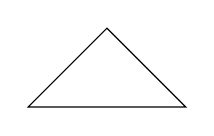
\begin{tikzpicture}
\draw (0,0) -- (1,1) 
   -- (2,0) -- cycle;
\end{tikzpicture}
\end{example}

其它常用的路径还包括:
\begin{itemize}
  \item 矩形、圆和椭圆:
\end{itemize}
\begin{example}
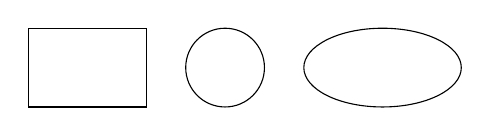
\begin{tikzpicture}
\draw (0,0) rectangle (1.5,1);
\draw (2.5,0.5) circle [radius=0.5];
\draw (4.5,0.5) ellipse
    [x radius=1,y radius=0.5];
\end{tikzpicture}
\end{example}

\begin{itemize}
  \item 直角、圆弧:
\end{itemize}
\begin{example}
\begin{tikzpicture}
\draw (0,0) |- (1,1);
\draw (1,0) -| (2,1);
\draw (4,0) arc (0:135:1);
\end{tikzpicture}
\end{example}

\begin{itemize}
  \item 二次和三次 B\'ezier 曲线,分别使用一个和两个控制点:
\end{itemize}
\begin{example}
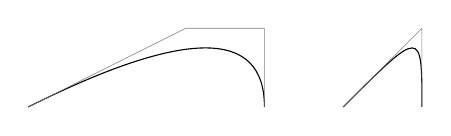
\begin{tikzpicture}
\draw (0,0) .. controls 
  (2,1) and (3,1) .. (3,0);
\draw (4,0) .. controls
  (5,1) .. (5,0);
\draw[help lines] (0,0)
  -- (2,1) -- (3,1) -- (3,0)
  (4,0) -- (5,1) -- (5,0);
\end{tikzpicture}
\end{example}

\begin{itemize}
  \item 网格、函数图像,网格可用 \texttt{step} 选项控制网格大小,函数图像用 \texttt{domain} 选项控制定义域:
\end{itemize}
\begin{example}
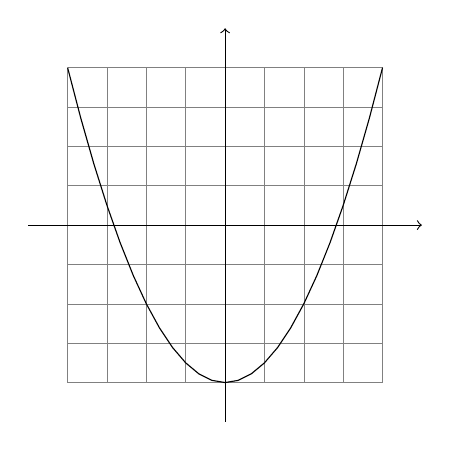
\begin{tikzpicture}
\draw[help lines,step=0.5] 
     (-2,-2) grid (2,2);
\draw[->] (-2.5,0) -- (2.5,0);
\draw[->] (0,-2.5) -- (0,2.5);
\draw[domain=-2:2] 
     plot(\x,{\x*\x -2});
\end{tikzpicture}
\end{example}

\subsection{\TikZ\ 绘图命令和参数}\label{subsec:tikz-draw}

\cmdindex[tikz]{draw,fill,filldraw}
除了 \cmd{draw} 命令之外,\TikZ\ 还提供了 \cmd{fill} 命令用来填充图形,\cmd{filldraw} 命令则同时填充和描边。
除了矩形、圆等现成的闭合图形外,\cmd{fill} 和 \cmd{filldraw} 命令也能够填充人为构造的闭合路径。
\begin{command}
\cmd{draw}\oarg*{\ldots} \Arg{path}; \quad
\cmd{fill}\oarg*{\ldots} \Arg{path}; \\
\cmd{filldraw}\oarg*{\ldots} \Arg{path}; 
\end{command}

绘图参数可作为可选参数用在 \env{tikzpiture} 环境或 \cmd{tikz} 命令时,参数会影响到所有具体的绘图命令;
用在单个绘图命令 \cmd{draw}、\cmd{filldraw} 等时,只对这个命令起效。

\TikZ 有数不清的绘图参数,这些参数令 \TikZ\ 能够绘制丰富多彩的图像,同时也令 \TikZ\ 易学难精。
本手册仅总结常用的一些绘图参数,见表 \ref{tbl:tikz-options}。

\begin{table}[htp]
\caption{\TikZ\ 常用的一些绘图参数。}\label{tbl:tikz-options}
\small
\hrule
\begin{itemize}
  \item \texttt{color=\Arg{color}} \par
  为线条(\cmd{draw})或填充(\cmd{fill})指定颜色,\Arg{color} 使用颜色名或是 \pkg{xcolor} 的混合颜色语法。
  往往可以不写 \texttt{color=} 直接写颜色名称。
  \item \texttt{fill=\Arg{color} / draw=\Arg{color}} \par
  分别给 \cmd{filldraw} 指定填充和描边的颜色。也可分别给 \cmd{fill} 和 \cmd{draw} 命令使用。
  不带参数直接使用 \texttt{fill} 和 \texttt{draw},相当于用默认颜色。
\end{itemize}
\hrule
\begin{itemize}
  \item \texttt{line width=\Arg{length}} \par
  指定线条粗细为 \Arg{width}。默认为普通线宽 0.4pt。
  \item \texttt{thin / semithick / thick / \ldots} \par
  指定线条粗细为预定义的某个类型,默认为 \texttt{thin}。总共有七种预定义的类型:
  \texttt{ultra thin},\texttt{very thin},\texttt{thin},\texttt{semithick},\texttt{thick},
  \texttt{very thick},\texttt{ultra thick}。
  \item \texttt{help lines} \par
  指定线条为辅助线,相当于 \texttt{line width=0.2pt,gray}。
  \item \texttt{solid / dashed / dotted / dash dot / dash dot dot / \dots} \par
  指定线条类型(实现、虚线等)。
  \item \texttt{rounded corners} \par
  将路径转向处绘制成圆角。可写成 \texttt{rounded corners=\Arg{radius}} 使用给定的半径。
\end{itemize}
\hrule
\begin{itemize}
  \item \texttt{-> / -< / -to / -latex / -stealth / \ldots} \par
  指定路径终点的箭头种类。
  \item \texttt{<- / >- / to- / latex- / -stealth / \ldots} \par
  指定路径起点的箭头种类。起点和终点的箭头可以搭配,如 \texttt{<->} 或者 \texttt{latex-to} 等。
\end{itemize}
\hrule
\begin{itemize}
  \item \texttt{scale=\Arg{scale}} \par
  指定整个图像或某个路径的缩放比例。
  \item \texttt{xshift=\Arg{length} / yshift=\Arg{length}} \par
  指定整个图像或某个路径相对于原位置的水平/垂直位移。
  \item \texttt{rotate=\Arg{angle}} \par
  指定整个图像或某个路径旋转一定角度。
\end{itemize}
\hrule
\end{table}

\subsection{\TikZ\ 文字结点}\label{subsec:tikz-node}

\cmdindex[tikz]{node}
\TikZ\ 用 \cmd{node} 命令绘制文字结点:
\begin{command}
\cmd{node}\oarg{options} \texttt{(\Arg{name})} \texttt{at (\Arg{coordinate})} \marg{text}\texttt{;}
\end{command}
\begin{example}
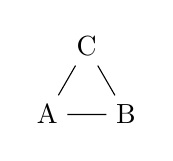
\begin{tikzpicture}
\node (A) at (0,0) {A};
\node (B) at (1,0) {B};
\node (C) at (60:1) {C};
\draw (A) -- (B) -- (C) -- (A);
\end{tikzpicture}
\end{example}

表 \ref{tbl:tikz-options} 中的参数可用于 \cmd{node} 命令的配置。除此之外,\cmd{node} 还有一些特定的参数,见表 \ref{tbl:tikz-node-options}。

\begin{table}[htp]
\caption{\TikZ\ 结点使用的一些绘图参数。}\label{tbl:tikz-node-options}
\small
\hrule
\begin{itemize}
  \item \texttt{anchor=\Arg{position}} \par
  指定结点的某个角落 \Arg{position} 位于给定的位置 \Arg{coordinate}。
  \item \texttt{center/ above / below / left / right / above left / \ldots} \par
  指定结点相对于 \Arg{coordinate} 的位置,\texttt{anchor=\Arg{position}} 的等效写法。\texttt{above} 相当于 \texttt{anchor=south},以此类推。
  带参数的形式 \texttt{above=\Arg{length}} 指定节点相对于 \Arg{coordinate} 的距离。
  \item \texttt{shape=\Arg{shape}} \par
  结点的形状,默认可用 \texttt{rectangle} 和 \texttt{circle},可省略 \texttt{shape=} 直接写。在导言区使用命令 
  \cmd{use\-tikz\-library}\marg*{shapes.geometric} 可用更多的形状。
  \item \texttt{inner sep=\Arg{length} / outer sep=\Arg{length}} \par
  结点边界向外和向内的额外距离。
  \item \texttt{minimum size=\Arg{length} / minimum height=\Arg{length} / minimum width=\Arg{length}} \par
  结点的最小大小或最小高度/宽度。
  \item \texttt{text=\Arg{color}} \par
  结点文字的颜色。
  \item \texttt{node font=\Arg{font command}} \par
  结点文字的字体,形如 \cmd{bfseries} 或 \cmd{itshape} 等。
\end{itemize}
\hrule
\end{table}

\cmd{node} 命令不仅为文字结点的位置命名(类似 \cmd{coordinate} 命令),在 \cmd{draw} 等命令中还可以使用某个结点的相对位置,
以“东南西北”的方式命名:

\begin{example}
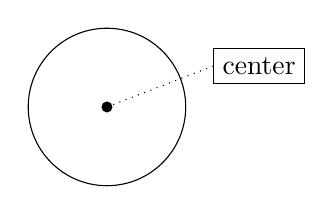
\begin{tikzpicture}
\draw (0,0) circle[radius=1];
\fill (0,0) circle[radius=2pt];
\node[draw] (P) at (15:2) {center};
\draw[dotted] (0,0) -- (P.west);
\end{tikzpicture}
\end{example}

另一种用法是在 \cmd{draw} 等命令的路径中使用 \texttt{node},不仅可以对某个位置标记节点,还能够对线标记:
\begin{example}
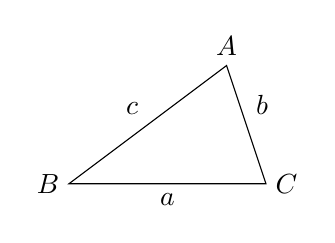
\begin{tikzpicture}
\draw (2,1.5) node[above] {$A$}
       -- node[above left]  {$c$}
    (0,0) node[left]  {$B$}
       -- node[below]       {$a$}
  (2.5,0) node[right] {$C$}
       -- node[above right] {$b$}
       cycle;
\end{tikzpicture}
\end{example}

除了 \cmd{node} 命令之外,\cmd{coordinate} 也可以通过参数为某个位置添加文字。
我们最后举一个较为复杂的例子,综合前面介绍过的各种路径、形状、文字结点和参数设置。

\begin{sourcecode}[htp]
\begin{Verbatim}
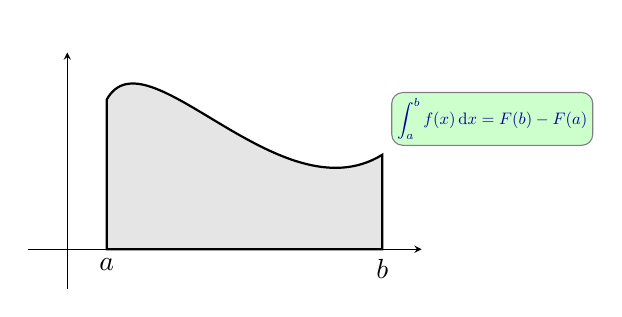
\begin{tikzpicture}
\draw[-stealth,line width=0.2pt] (-0.5,0) -- (4.5,0);
\draw[-stealth,line width=0.2pt] (0,-0.5) -- (0,2.5);
\coordinate (a)  at (0.5,1.9);
\coordinate (b)  at (4,1.2);
\coordinate[label=below:$a$] (a0) at (0.5,0);
\coordinate[label=below:$b$] (b0) at (4,0);
\filldraw[fill=gray!20,draw,thick] 
  (a0) -- (a) .. controls (1,2.8) and (2.7,0.4) .. (b) -- (b0) -- cycle;
\node[above right,outer sep=0.2cm, rounded corners,
  fill=green!20,draw=gray,text=blue!60!black,scale=0.6] 
  at (b) {$\displaystyle \int_a^b {f(x)\,\mathrm{d}x} = F(b) - F(a)$};
\end{tikzpicture}
\end{Verbatim}
\begin{center}
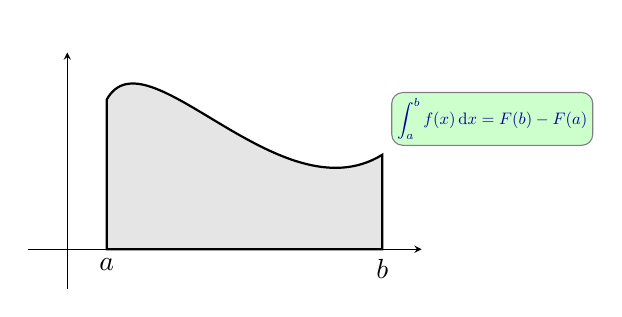
\begin{tikzpicture}
\draw[-stealth,line width=0.2pt] (-0.5,0) -- (4.5,0);
\draw[-stealth,line width=0.2pt] (0,-0.5) -- (0,2.5);
\coordinate (a)  at (0.5,1.9);
\coordinate (b)  at (4,1.2);
\coordinate[label=below:$a$] (a0) at (0.5,0);
\coordinate[label=below:$b$] (b0) at (4,0);
\filldraw[fill=gray!20,draw,thick] 
  (a0) -- (a) .. controls (1,2.8) and (2.7,0.4) .. (b) -- (b0) -- cycle;
\node[above right,outer sep=0.2cm, rounded corners,
  fill=green!20,draw=gray,text=blue!60!black,scale=0.6] 
  at (b) {$\displaystyle \int_a^b {f(x)\,\mathrm{d}x} = F(b) - F(a)$};
\end{tikzpicture}
\end{center}
\caption{\TikZ\ 绘图示例源代码和效果。}\label{code:tikz-example}
\end{sourcecode}

\endinput